%+++++++++++++++++++++++++++++++++++++++++++++++++++++++++++++++
% SUMMARY    : KNN, Regression, Scale Data and Classifier Function 
%            : University of Southern Maine 
%            : @james.quinlan
%            : Deiby Wu - Lecture 4
%+++++++++++++++++++++++++++++++++++++++++++++++++++++++++++++++
\section*{Objectives}
\begin{outline}
    \1 K-Nearest Neighbors (KNN)
    \1 Regression
    \1 Scale Data
    \1 ``Homework" Problems
    \1 Outline for KNN algorithm
    \1 Classifier Function
    \1 Class Code
\end{outline}

\rule[0.0051in]{\textwidth}{0.00025in}
% ----------------------------------------------------------------

\section{K-Nearest Neighbors (KNN)}

\textbf{KNN} is an algorithm that can be use for Regression and Classification tasks. Its function is to classify new data points
by checking what is nearby them as its names indicate.

This is how the data looks:\\
$Data = \{(x_1, y_1), (x_2, y_2), \dots, (x_n, y_n)\}$

where $x \in \mathbb{R}^p$

They look like a set of pairs where $x$ represent the features, while $y$ is the label that belongs to $x$.

In the classification case, $y$ is a discrete label, and in the regression case, $y$ is a real number.

% -----------------------------------------------------------------------------------------------

\section{Regression Case}

\subsection{Example of feature representation for a regression case}

\begin{center}
    \textbf{Predicting House Prices}
\end{center}

\vspace{-0.5cm}

\begin{align*}
    x &= \begin{bmatrix}
            \text{Sq. ft} \\
            \text{Dist to Ocean} \\
            \text{Dist to School} \\
            \vdots \\
         \end{bmatrix} \\\\\\
    y &= [325,000]
\end{align*}

Here the input feature $x$ consists of multiple attributes related to the house,
like the  square feet, the distance to the ocean, and the distance to school. The target
variable $y$ represents the price of the home.\\\\

\subsection{Example of use case for regression case}

For missing values on temperature for a particular city, instead of
taking the average of every city in the country, we consider the average
temperature of the 3 nearest cities. Let say we are trying to find the temperature
of a city in New Hampshire.

\begin{center}
    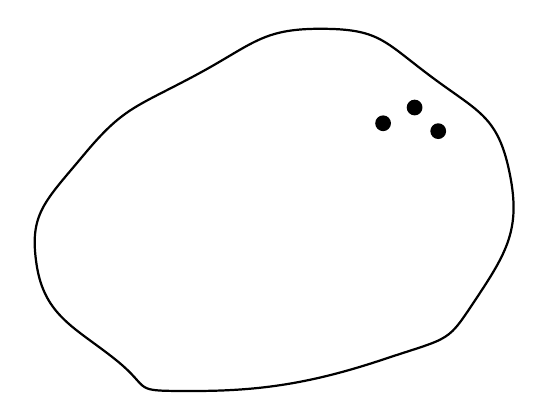
\begin{tikzpicture}
        \draw[thick] plot[smooth cycle, tension=0.9] coordinates {
            (0,0) (2.4,0.4) (3.6,1.2) (4,2.8) (3,4) (1.6,4.6) 
            (0,4) (-1.4,3) (-2,1.6) (-1,0.4)
        };

        \fill (2.4, 3.4) circle (0.1);
        \fill (2.8, 3.6) circle (0.1);
        \fill (3.1, 3.3) circle (0.1);

    \end{tikzpicture}
\end{center}

Let's assume this dissorted circle is the map of The United States, and we are trying
to find the temperature of a city in New Hampshire. The three dots inside the circle
represent other cities near New Hampshire. We take the temperature of those 3 dots (cities),
and then we average them to find the missing temperature from the city in New Hampshire. That's one
way of doing it.

\subsection{Dot Product and Cross-Validation in Regression}

\begin{center}
    \textbf{Understanding Dot Product and Cross-Validation for House Price Prediction}
\end{center}

\vspace{-0.5cm}

The dot product is a fundamental operation in linear regression, where the input feature vector \( x \) is multiplied by the learned weight vector \( w \) to predict the target \( y \). Mathematically, this can be written as:

\begin{align*}
    x &= \begin{bmatrix}
            x_0 \\ x_1 \\ x_2
         \end{bmatrix} =
         \begin{bmatrix}
            \text{Sq. ft} \\
            \text{Dist to Ocean} \\
            \text{Dist to School}
         \end{bmatrix}, \quad
    w = \begin{bmatrix}
            w_0 \\ w_1 \\ w_2
         \end{bmatrix}
\end{align*}

The predicted house price is computed using the dot product:

\begin{align*}
    y_{\text{pred}} &= w \cdot x \\
    &= \sum_{i=0}^{2} w_i x_i
\end{align*}


where:
- \( w_0, w_1, w_2 \) are learned weights,
- \( y_{\text{pred}} \) is the predicted house price.

This operation essentially performs a \textbf{weighted sum of the input features} to generate the prediction.

\begin{center}
\resizebox{!}{5cm}{ % Adjust height, width auto-scales
    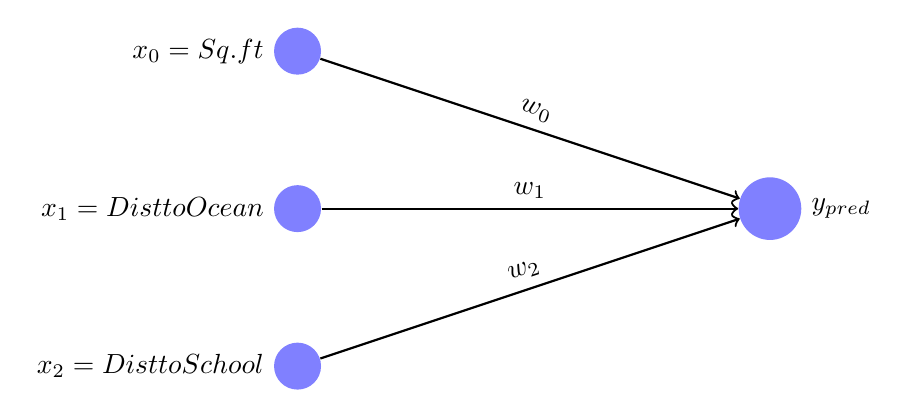
\begin{tikzpicture}
        % Input nodes (features)
        \node[circle, fill=blue!50, inner sep=6pt, label=left:{$x_0 = \text{Sq. ft}$}] (x0) at (0,6) {};
        \node[circle, fill=blue!50, inner sep=6pt, label=left:{$x_1 = \text{Dist to Ocean}$}] (x1) at (0,4) {};
        \node[circle, fill=blue!50, inner sep=6pt, label=left:{$x_2 = \text{Dist to School}$}] (x2) at (0,2) {};

        % Output node (prediction)
        \node[circle, fill=blue!50, inner sep=8pt, label=right:{$y_{\text{pred}}$}] (output) at (6,4) {};

        % Weights and connections
        \draw[thick, ->] (x0) -- node[midway, above, sloped] {\(w_0\)} (output);
        \draw[thick, ->] (x1) -- node[midway, above, sloped] {\(w_1\)} (output);
        \draw[thick, ->] (x2) -- node[midway, above, sloped] {\(w_2\)} (output);

    \end{tikzpicture}
}
\end{center}


\textbf{Cross-Validation for Model Generalization}

To ensure that our model generalizes well to unseen data, we use \textbf{k-fold cross-validation}, which consists of the following steps:

\begin{enumerate}
    \item Split the dataset into \( k \) subsets (folds).
    \item Train the model on \( k-1 \) folds while leaving one fold for validation.
    \item Repeat this process \( k \) times, using a different fold for validation each time.
    \item Average the performance across all \( k \) runs to obtain a reliable estimate of model accuracy.
\end{enumerate}

% -----------------------------------------------------------------------------------------------

\section{Preprocessing} 

\subsection{Scale Data}
Scaling data is important in machine learning algorithm to maintain consistency.
Some features might have large values while other have small, meaning that models will
be more biased to the larger values. So, when they are in the same range, it is easier for
models to compare the data impact on the result. For example, when dealing with distances metrics, 
1000 miles compared to 50 fts, the 1000 miles will completely dominated the distance calculation, so, it
is always necessary to scale this type of data.

\subsection{Scaling Techniques}
\begin{outline}[enumerate]
\1 \textbf{Standarize}

\[
x_i^{\prime} = \frac{x_i - \bar{x}}{\sigma} = Z
\]

\begin{itemize}
    \item $x_i^{\prime}$: the new data point  
    \item $x_i$: the old data point  
    \item $\sigma$: the standard deviation
    \item $\bar{x}$: mean of entire column of values
    \item $Z$: $Z$-score
\end{itemize}

Where:

\begin{align*}
x_i &= \begin{bmatrix}
        x_{1} \\
        x_{2} \\
        x_{3} \\
        \vdots \\
        x_{p}
        \end{bmatrix} \\
\end{align*}

For this standarize formula, we take the original values ($x_i$), subtract it with the mean of the
entire column ($\bar{x}$), to later divide it with the standard deviation ($\sigma$), we would get the
Z-score. This is one way of scaling data.


\1 \textbf{Normalize (min max scaler)}

For this scaling technique, we take the values of $x$, and then map them to the interval from $0$ to $1$:

\[
    x \rightarrow [0,1]
\] 

For example, we have values that ranges from $2$ to $10$, then we would want to map $2$ to $0$, and $10$ to $1$.

\[
    [2,10] \rightarrow [0,1]
\] 

\begin{center}
    \begin{tikzpicture}
        % Setup the structure
        \draw[->, thick] (-1, 0) -- (6, 0) node[right] {$x$};
        \draw[->, thick] (0, -1) -- (0, 6) node[above] {$y$};

        % Fill up with a grid
        \draw[gray, dotted] (-1, -1) grid (6, 6);

        % Draw the lines that connect [2,10] to [0,1]
        \draw[thick] (1,0) -- (1,1) -- (0,1);
        \draw[thick] (5,0) -- (5,5) -- (0,5);

        % Draw dotted lines in between the range of [2,10] to [0,1]j
        \draw[dashed] (2,0) -- (2,2) -- (0,2);
        \draw[dashed] (2.5,0) -- (2.5,2.5) -- (0,2.5);
        \draw[dashed] (3.4,0) -- (3.4,3.4) -- (0,3.4);
        \draw[dashed] (4.5,0) -- (4.5,4.5) -- (0,4.5);

        % Label the coordinates
        \node[below] at (1, 0) {2};
        \node[below] at (5, 0) {10};
        \node[below] at (-0.4, 1.2) {0};
        \node[below] at (-0.4, 5.2) {1};
    \end{tikzpicture} \\
\end{center}

As we can see in the graph, we mapped $2$ to $0$, and $10$ to $1$, and they can be denoted by the solid lines,
while the dashed lines represent a number in between $2$ and $10$ that connect to a value in between $0$ and $1$.

\end{outline}

\section{Exploration (XPL) Problems}
\begin{outline}[enumerate]

    \1  Code the Standarize Scaler formula. \\

    \1  Write down the formula for linear transformation, and then code it. e.g.$[2,10]$ $\rightarrow$ $[0,1]$ and anything in between.\\

    \1 Write a linear transformation that maps $[a,b]$ to $[c,d]$ (draw a line for them). \\

\end{outline}

% -----------------------------------------------------------------------------------------------

\section{Outline for the KNN algorithm}
\begin{outline}

    \1  Given a dataset: $D=\{x_i,y_i\}$

    \1  Compute the distance from new point $x_t$ that is not in the set $D$, to every  $x_i$

    \1  Sort distances

    \1  Select first $K$ of the sorted distances

    \1  If \textbf{Classification} problem, take the mode of labels $y_1, y_2, y_3 ... y_k$, else, for \textbf{Regression}
        problem, take the mean of labels $y \in \mathbb{R} \rightarrow y_1, y_2, y_3 ... y_k$ (as an alternative, using median could be
        ideal in some cases since it ignore outliers)

\end{outline}

$x_t$ is a test point\\

$K \subseteq D$ \\

$|K| = k$, where $|K|$ represent the number of elements in that subset\\

$\forall(x^{\prime},y^{\prime}) \in D \hspace{1 mm} \backslash \hspace{1 mm} K$, for every point that is outside of $K$,
the distance from the test point to all the points outside of $K$ have to be bigger than the maximum distance inside of $K$.

\[
    d(x^{\prime},y^{\prime}) \geq max \hspace{1 mm} d \hspace{1 mm} (x_t, x^{\prime\prime})
\]


\begin{center}
    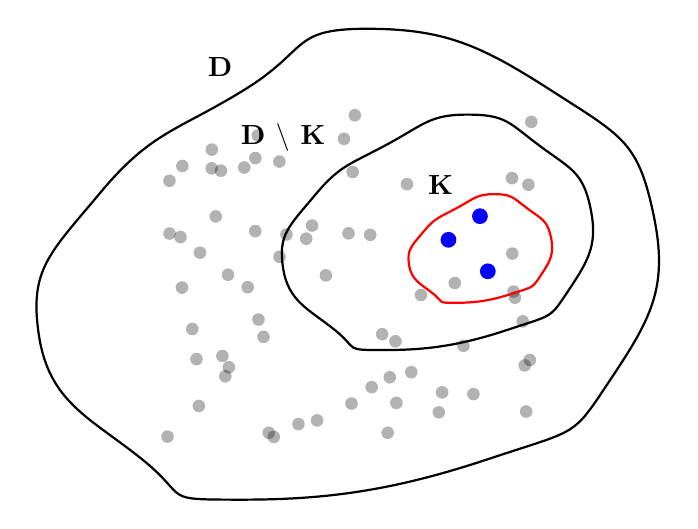
\begin{tikzpicture}
        % Outer circle
        \draw[thick, scale=1.3] plot[smooth cycle, tension=0.9] coordinates {
            (0,0) (2.4,0.4) (3.6,1.2) (4,2.8) (3,4) (1.2,4.6) 
            (0,4) (-1.4,3) (-2,1.6) (-1,0.4)
        };

        % Label for Outer circle
        \node at (-0.3,5.5) {\textbf{D}};

        \foreach \i in {1,...,65} {
            \fill[black, opacity=0.3] 
            ({1.3 + 2.4*rand}, {2.8 + 2.16*rand}) circle (0.08);
        }

            % Inner circle
            \begin{scope}[shift={(1.8,1.9)}, scale=1.3]
                \draw[thick] plot[smooth cycle, tension=0.9] coordinates {
                    (0,0) (1.2,0.2) (1.8,0.6) (2,1.4) (1.5,2) (0.8,2.3) 
                    (0,2) (-0.7,1.5) (-1,0.8) (-0.5,0.2)
                };
            \end{scope}

            % Label for Inner circle
            \node at (0.5,4.6) {\textbf{D $\backslash$ K}};

                % Circle inside inner circle
                \begin{scope}[shift={(2.7,2.5)}, scale=0.6]
                    \draw[red, thick] plot[smooth cycle, tension=0.9] coordinates {
                        (0,0) (1.2,0.2) (1.8,0.6) (2,1.4) (1.5,2) (0.8,2.3) 
                        (0,2) (-0.7,1.5) (-1,0.8) (-0.5,0.2)
                    };
                \end{scope}
                
                % Label for circle inside Inner circle
                \node at (2.5,4) {\textbf{K}};

        % Test point
        % \fill[purple] (-0.4, 2) circle (0.1);
        
        % K=3 points
        \fill[blue] (2.6, 3.3) circle (0.1);
        \fill[blue] (3, 3.6) circle (0.1);
        \fill[blue] (3.1, 2.9) circle (0.1);

    \end{tikzpicture}
\end{center}

In the graph shown above, $D$ represents the whole data points, $D$ $\backslash$ $K$
represent the points outside of $K$, and $K$ contains its own points that is also part of $D$.
There are three blue dots ($K$=3) inside of $K$ surrounded by a red circle. This three
dots are the 3 nearest neighbors used for classification or regression task in KNN. So,
given a new test point, KNN calculates the distance between this new test point, and every point in the dataset.
It then selects the K closest point as its neighbors (K=3 in this case), and then, it would either assign a class
or predict a value depending of the task to that new data point by comparing the proximity of the data point to the
nearest neighbor.

% -----------------------------------------------------------------------------------------------

\section{Classifier Function}

\[
    h(x) = \operatorname*{argmax}\limits_{\substack{j = \{1,2,\dots,m\}}} \hspace{3mm} \sum_{i=N_k} I_{cj}(y_i)
\]

This can also be called \textbf{mode function}, which is used to find the value that appears most frequently in the dataset.

\[
I_{cj} (y_i) = 
\begin{cases}
    1 & y_i = c_j\\
    0 & y_i \neq c_j
\end{cases}
\]

This is a flag function, that will determine if a value is true or false, and the classifier function will accumulate all of
those, and output the mode.

\subsection{argmax and argmin}

\begin{center}
    \begin{tikzpicture}
        % Setup the structure
        \draw[->, thick] (-1, 0) -- (8.5, 0) node[right] {$$};
        \draw[->, thick] (0, -2) -- (0, 7.5) node[above] {$$};

        % Random curves
        \draw[domain=0:8, smooth, variable=\x, thick, blue] 
            plot ({\x}, {4 - 2*cos(deg(\x - 2)) + sin(deg(3*\x)) + 0.5*sin(deg(4*\x))});

        \draw[dashed, red] (0.34,0) -- (0.34,5.55);
        \fill[red] (0.34,5.55) circle (0.1);
        \node[below] at (0.34, 0) {$x_1$};

        \draw[dashed, red] (1.47,0) -- (1.47,1.2);
        \fill[red] (1.47,1.2) circle (0.1);
        \node[below] at (1.47, 0) {$x_2$};

        \draw[dashed, red] (2.4,0) -- (2.4,2.9);
        \fill[red] (2.4,2.9) circle (0.1);
        \node[below] at (2.4, 0) {$x_3$};

        \draw[dashed, red] (4.94,0) -- (4.94,7.1);
        \fill[red] (4.94,7.1) circle (0.1);
        \node[below] at (4.94, 0) {$x_4$};

        \draw[dashed, red] (5.94,0) -- (5.94,4.1);
        \fill[red] (5.94,4.1) circle (0.1);
        \node[below] at (5.94, 0) {$x_5$};

        \draw[dashed, red] (6.64,0) -- (6.64,5.5);
        \fill[red] (6.64,5.5) circle (0.1);
        \node[below] at (6.64, 0) {$x_6$};

        \draw[dashed, red] (7.73,0) -- (7.73,1.2);
        \fill[red] (7.73,1.2) circle (0.1);
        \node[below] at (7.73, 0) {$x_7$};


    \end{tikzpicture} \\
\end{center}


Given a function $f(x)$, try to find the min and max for the function.
We take the derivative of the function and set it to zero ($f^{\prime}(x) = 0$).
A reason for that is because max and min can only occur when the derivate is set to zero, and
then we solve for $x$. In the graph above, we can see different sets of $x$ that could 
be used to find the min and max of the function. If we plug $x_4$ to the function, $f(x_4)$,
we will find the \textbf{argmax}, which is the $x$ value that makes the function maximum. This concept
also applies to find the \textbf{argmin}, where we look for the $x$ value (in this case $x_2$), which will make
the function minimum.\\


\begin{center}
    \begin{tikzpicture}
        % Setup the structure
        \draw[->, thick] (-1, 0) -- (7.5, 0) node[right] {$$};
        \draw[->, thick] (0, -1) -- (0, 7.5) node[above] {$$};

        % Plot curve
        \draw[domain=0:7, smooth, variable=\x, thick, blue] 
            plot ({\x}, {2*sin(deg(\x)) + 4});

        % Argmax
        \draw[dashed, red] (1.57,0) -- (1.57,6);
        \fill[red] (1.57,6) circle (0.1);
        \node[below] at (1.57, 0) {$argmax$};

        % Argmin
        \draw[dashed, purple] (4.71,0) -- (4.71,2);
        \fill[purple] (4.71,2) circle (0.1);
        \node[below] at (4.71, 0) {$argmin$};

    \end{tikzpicture} \\
\end{center}

As shown in the graph above, the argmax is the input value ($x$) to produce the maximum
output value for the function. We must remember that $f(x) = y$, so, the \textbf{argmax}
will produce the highest $y$ value.\\\\


\subsection{Example of mode function}

Let say we have a new data point as shown in the graph below represented by a red dot, and there
are already a set of 9 y's values:

\begin{center}
    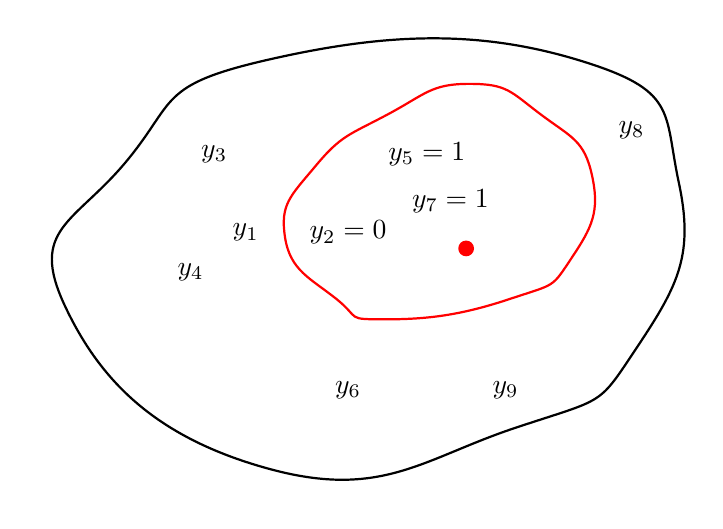
\begin{tikzpicture}
        % Outer circle
        \draw[thick, scale=1.3] plot[smooth cycle, tension=0.9] coordinates {
            (0,0) (2.4,0.4) (3.6,1.2) (4,2.8) (3,4) 
            (0,4) (-1.4,3) (-2,1.6) 
        };

        % Label for inner circle
        \node at (1,3) {$y_2 = 0$};
        \node at (2,4) {$y_5 = 1$};
        \node at (2.3, 3.4) {$y_7 = 1$};
        \fill[red] (2.5,2.8) circle (0.1);

        % label for outer circle
        \node at (-0.3,3) {$y_1$};
        \node at (-0.7,4) {$y_3$};
        \node at (-1,2.5) {$y_4$};
        \node at (4.6,4.3) {$y_8$};
        \node at (1,1) {$y_6$};
        \node at (3,1) {$y_9$};


            % Inner circle
            \begin{scope}[shift={(1.5,1.9)}, scale=1.3]
                \draw[red, thick] plot[smooth cycle, tension=0.9] coordinates {
                        (0,0) (1.2,0.2) (1.8,0.6) (2,1.4) (1.5,2) (0.8,2.3) 
                        (0,2) (-0.7,1.5) (-1,0.8) (-0.5,0.2)
                    };
            \end{scope}


    \end{tikzpicture}
\end{center}

Let say we assign $K = 3$, then it will select the nearest neighbors to that new data point.
As seen in the graph, $y_2$ has a value of 0, $y_5$ is 1, and $y_7$ is 1 (0 and 1 are classes in this case), and
they are the closest to the new data point. Later, we find the mode, and since the class 1 was the predominant one,
the new data point would be assigned to be class 1.\\
One important thing to do, if there are let say 2 classes, $K$ should not be a multiple of 2 to break ties, so $K$ could be
3 or 5 or 7. This concept also applies for cases where there are 3 classes, we avoid choosing a $K$ that is a multiple of 3.

% -----------------------------------------------------------------------------------------------
\section{Class Code}
Language: Julia
\begin{minted}[frame=lines, framesep=2mm]{julia}
# Installing the necessary packages
using Pkg
Pkg.add("RDatasets")
Pkg.add("MLJBase")
Pkg.add("Distances")

# Import packages for data handling
using Distances
using RDatasets

# Load the Iris dataset from the RDatasets package
iris = dataset("datasets", "iris")

# Extract the first four columns of the Iris dataset as a matrix (feature variables)
X = Matrix(iris[:,1:4])

# Extract the target variable from the Iris dataset and store it in y
y = iris.Species

# Convert the target variable into binary labels:  
# Assign 1 to "setosa" and -1 to all other species  
y = @. ifelse(iris.Species == "setosa", 1, -1)

# Get the unique class labels in the target variable
c = unique(y)

# Find the most frequent class label in y (this is mode technically)
c[argmax(map(i -> sum(y .== c[i]), 1:lastindex(c)))]
\end{minted}
